% SPDX-FileCopyrightText: 2025 Jorge Teixeira Crespo <jorge.teixeira@udc.es>
%
% SPDX-License-Identifier: GPL-2.0-or-later

\chapter{Implementation}
\label{chap:implementation}

\lettrine{T}{he} deployment of the new infrastructure begins with provisioning a dedicated physical server hosted at Hetzner\cite{hetzner-server-bidding}. This server replaces the previous GPUL machines (\texttt{gpulino} and \texttt{gpulon}), and is named \texttt{gpulux}, reflecting its role as the unified and modernized core system.

\section{Installation and Base System}

The base system was installed using Hetzner's \texttt{installimage}\cite{hetzner-installimage} provisioning tool. The configuration focused on separating system and data storage for flexibility and performance.

Debian was chosen as the operating system, a decision rooted in its renowned stability for server roles and the human merits of its contributors. These values are chronicled by Krafft in \emph{The Debian System}\cite{krafft2005debian}. This choice also honors GPUL's historical ties to Debian and the contributions of past board members who are consolidated Debian maintainers\cite{berto-debian-page}.

\subsection*{installimage Configuration}

The installation was performed on the two 512 GB disks using software RAID 1 to ensure redundancy. The two 2 TB disks were left untouched during provisioning and later configured manually.

The following snippet shows the \texttt{installimage} configuration file:

\begin{lstlisting}[caption={Configuration used by Hetzner's installimage script to deploy Debian on gpulux}]
DRIVE1 /dev/nvme2n1
DRIVE2 /dev/nvme3n1
SWRAID 1
SWRAIDLEVEL 1
HOSTNAME gpulux
USE_KERNEL_MODE_SETTING yes
PART swap  swap   32G
PART /boot ext3  1024M
PART /     ext4   all
IMAGE /root/.oldroot/nfs/install/../images/ Debian-1208-bookworm-amd64-base.tar.gz
\end{lstlisting}

This setup results in the following RAID arrays:

\begin{itemize}
  \item \texttt{/dev/md0} - 32 GB swap
  \item \texttt{/dev/md1} - 1 GB \texttt{/boot}
  \item \texttt{/dev/md2} - 440 GB for root filesystem
\end{itemize}

\subsection*{Post-Install Configuration}

After installation, the two 2 TB NVMe drives (\texttt{/dev/nvme0n1} and \texttt{/dev/nvme1n1}) were manually configured into a new RAID 1 array, \texttt{/dev/md3}. For security hardening, SSH access for the \texttt{root} user was disabled, and a new admin user, \texttt{tei*****}, was created with \texttt{sudo} privileges. Access for this user is granted via SSH with public key authentication, as password authentication has been disabled server-wide.

\section{Containerization with Incus}

Incus is not included in the standard Debian 12 (Bookworm) repositories, so it must be installed from the \texttt{bookworm-backports} repository. The backports provide newer software versions that are scheduled for inclusion in future Debian releases, in this case, Debian 13 (Trixie).

To enable the backports, a new APT source file is created, including both the official Debian mirror and the Hetzner mirror for optimized download speeds.

\begin{lstlisting}[language=bash,caption={APT sources list enabling the bookworm-backports repository}]
deb http://mirror.hetzner.com/debian bookworm-backports main
deb http://deb.debian.org/debian bookworm-backports main
\end{lstlisting}

With the backports repository configured, Incus can be installed. Only the \texttt{incus-base} package is installed, as this provides the necessary tools for managing containers without the overhead of full virtual machine support. This approach aligns with the current plan, and support for VMs can be added later if needed.

\begin{lstlisting}[language=bash,caption={Commands to install the Incus server from Debian backports}]
sudo apt update
sudo apt install incus-base/bookworm-backports
\end{lstlisting}

To manage Incus, users must be added to the \texttt{incus-admin} group. The administrative user, \texttt{tei*****}, was added to this group.

\subsection*{Initial Incus Configuration}

Incus was initialized using the \texttt{incus admin init} command. The key configuration choices from the interactive setup are summarized below:
\begin{itemize}
    \item \textbf{Mode:} Standalone (non-clustered).
    \item \textbf{Storage Pool:} A new BTRFS storage pool named \texttt{default} was created on the dedicated data RAID array (\texttt{/dev/md3}).
    \item \textbf{Network:} A new local network bridge, \texttt{incusbr0}, was configured with the IPv4 subnet \texttt{10.42.0.1/24} and NAT enabled. IPv6 was disabled internally for this bridge.
    \item \textbf{Remote Access:} The Incus server is not exposed over the network.
    \item \textbf{Image Management:} Automatic updates for stale cached images were enabled.
\end{itemize}

\section{Monitoring Stack}

With the Incus environment established, the next step is to create containers to host the various services that will run on the new infrastructure. Each service, or group of related services, is isolated within its own container, providing a clean and manageable separation of concerns.

The first container to be created is for the monitoring stack. This stack is a critical component of the new infrastructure, providing insights into the health and performance of the host system and the services it runs.

\subsection*{Monitoring Container}

A new container named \texttt{monitoring} is launched using the official Debian 12 image. The following command is used:

\begin{lstlisting}[language=bash,caption={Command to create the monitoring container from a Debian 12 image}]
incus launch images:debian/12 monitoring
\end{lstlisting}

Once the container is running, it is possible to get an interactive shell inside it to perform administrative tasks. This is achieved with the \texttt{exec} command:

\begin{lstlisting}[language=bash,caption={Command used to obtain a shell inside the monitoring container}]
incus exec monitoring -- bash
\end{lstlisting}

Inside the \texttt{monitoring} container, a full monitoring stack is deployed. This stack consists of three key components:

\begin{itemize}
    \item \textbf{Prometheus:} For collecting and storing time-series data (metrics).
    \item \textbf{Loki:} For collecting and storing logs.
    \item \textbf{Grafana:} For visualizing data from both Prometheus and Loki.
\end{itemize}

\subsection*{Prometheus Configuration}

Prometheus was installed following the official documentation\cite{prometheus-getting-started} and configured to scrape both itself and the Incus host metrics:

\begin{lstlisting}[caption={Prometheus configuration scraping metrics from itself and the Incus host}]
scrape_configs:
  - job_name: "prometheus"
    static_configs:
      - targets: ["localhost:9090"]
  - job_name: "incus"
    metrics_path: '/1.0/metrics'
    scheme: 'https'
    tls_config:
      insecure_skip_verify: true
    static_configs:
      - targets: ['10.42.0.1:8444'] # internal incus gw addr
\end{lstlisting}

The host was previously configured to expose metrics without authentication using:

\begin{lstlisting}[language=bash]
incus config set core.metrics_address=:8444
incus config set core.metrics_authentication=false
\end{lstlisting}

\subsection*{Loki, Grafana and Journal Logs Collection}

Loki and Grafana were installed in the \texttt{monitoring} container following their official documentation\cite{grafana-install-debian}. Grafana's configuration is managed via its web UI, so it maintains its default settings post-installation.

Loki was configured to store logs on the container's filesystem in the \texttt{/data/loki} directory. A retention period of 744 hours (approximately one month) was set, after which older logs are automatically purged. It was made accessible from the host using a proxy device, which allows requests from the host's loopback interface to reach the Loki instance:

\begin{lstlisting}[language=bash]
incus config device add monitoring loki-proxy proxy \
  listen=tcp:127.0.0.1:3100 connect=tcp:127.0.0.1:3100
\end{lstlisting}

Grafana Alloy, installed on the host following official documentation\cite{grafana-alloy-install}, forwards logs from the system journal to Loki. The configuration\cite{grafana-alloy-config-example} extracts key metadata such as unit name, boot ID, transport, and priority level:

\begin{lstlisting}[caption={Grafana Alloy configuration forwarding systemd journal logs to Loki}]
loki.source.journal "all" {
  relabel_rules = discovery.relabel.journal_relabel.rules
  forward_to    = [loki.write.local.receiver]
}

discovery.relabel "journal_relabel" {
  targets = []

  rule {
    source_labels = ["__journal__systemd_unit"]
    target_label  = "unit"
  }

  # ...
}

loki.write "local" {
  endpoint {
    url = "http://127.0.0.1:3100/loki/api/v1/push"
  }
}
\end{lstlisting}

Additionally, Incus is configured to export internal events (e.g., instance start/stop, snapshot creation) directly to Loki\cite{incus-loki-api}:

\begin{lstlisting}[language=bash]
incus config set loki.api.url=http://127.0.0.1:3100
incus config set loki.instance=incus
\end{lstlisting}

\subsection*{Reverse Proxy Setup with Caddy}

To expose web services to the internet, a lightweight container named \texttt{proxy} was created using Alpine Linux. Caddy was installed to act as a reverse proxy. While it will eventually handle all public-facing services, its initial configuration is limited to exposing the Grafana dashboard.

\begin{lstlisting}[language=bash,caption={Commands used to set up the Caddy reverse proxy container}]
incus launch images:alpine/edge proxy
incus exec proxy -- apk add --no-cache caddy
incus file push Caddyfile proxy/etc/caddy/Caddyfile
incus exec proxy -- rc-service caddy start
incus exec proxy -- rc-update add caddy default

incus config device add proxy http80  proxy \
  listen=tcp:0.0.0.0:80  connect=tcp:127.0.0.1:80
incus config device add proxy http443 proxy \
  listen=tcp:0.0.0.0:443 connect=tcp:127.0.0.1:443
\end{lstlisting}

The last two commands add Incus proxy devices\cite{incus-proxy-device} to the \texttt{proxy} container. These devices forward traffic from the public IP addresses on the host to a port inside the container. Specifically, all traffic arriving at port 80 (HTTP) and 443 (HTTPS) on the host's public network interfaces is redirected to the corresponding ports on the container's loopback interface, where Caddy is listening. The Caddyfile used is as follows:

\begin{lstlisting}[caption={Caddyfile configuration used to expose Grafana through the reverse proxy}]
grafana.gpulux.org {
  reverse_proxy monitoring:3000
}
\end{lstlisting}

\subsection*{Grafana Usage}

Grafana was accessed using the configured domain. After creating a user, community dashboards for Prometheus and Incus were imported. The Incus dashboard provides a comprehensive overview of the host's performance, displaying real-time metrics such as CPU and memory usage, network traffic, and disk I/O at project and instance level. This allows for quick identification of resource-intensive instances and overall system health monitoring.

The integration with Loki enables deep exploration of system logs. Logs from the system journal are collected and enriched with metadata labels, providing structured records for debugging and security monitoring. For example, SSH authentication failures can be isolated and analyzed with a simple query, making it easy to spot suspicious activity.


\section{Email Server with Mailcow}

Although not discussed in the technology selection chapter---as it is a dependency for other services rather than a primary service itself---a robust email server is a critical requirement for the new infrastructure. It is needed by services like Grafana and Passbolt to send alerts and notifications, and is essential for operating the mailing lists. Mailcow was selected for this role due to its widespread adoption and positive reputation in the open-source self-hosting community. As a complete mail server suite based on Docker, it provides a powerful foundation that will also serve as the Mail Transfer Agent (MTA) for the community's mailing lists, which will be managed by Mailman 3.

\subsection*{Mailcow Container Setup}

To maintain isolation and simplify management, Mailcow is deployed within its own dedicated Incus container. As Mailcow relies on Docker and Docker Compose for its operation, the container needs to be configured to support nested virtualization\cite{incus-faq-docker-nesting}. A new container named \texttt{mailcow} is launched from the Debian 12 image.

\begin{lstlisting}[language=bash,caption={Commands to create and configure the Mailcow container}]
incus launch images:debian/12 mailcow
incus config set mailcow security.nesting=true
incus config set mailcow security.privileged=true
\end{lstlisting}

The \texttt{security.nesting} flag enables the container to run its own containerization environment, while \texttt{security.privileged} is required for Mailcow to manage the networking stack correctly. Inside the container, Docker is installed following the official Docker documentation.

A critical step in deploying an email server on a cloud provider like Hetzner is ensuring that outgoing email ports are not blocked. By default, Hetzner blocks these ports to prevent spam. A support ticket was opened to request the unblocking of these ports for \texttt{gpulux}'s IP address.

To allow external access to Mailcow's services, several ports must be forwarded from the host to the container. This is achieved using Incus proxy devices, which redirect traffic from the host's public IP to the container. Table~\ref{tab:mailcow-ports} lists the required ports\cite{mailcow-prerequisites}.

\begin{table}[H]
    \centering
    \rowcolors{2}{white}{udcgray!25}
\caption{Ports forwarded to the Mailcow container}
    \label{tab:mailcow-ports}
    \begin{tabular}{lll}
        \rowcolor{udcpink!25}
        \textbf{Service} & \textbf{Protocol} & \textbf{Port} \\
        \hline
        Postfix SMTP & TCP & 25 \\
        Dovecot POP3 & TCP & 110 \\
        Dovecot IMAP & TCP & 143 \\
        Postfix SMTPS & TCP & 465 \\
        Postfix Submission & TCP & 587 \\
        Dovecot IMAPS & TCP & 993 \\
        Dovecot POP3S & TCP & 995 \\
        Dovecot ManageSieve & TCP & 4190 \\
    \end{tabular}
\end{table}

The commands to create these proxy devices follow a similar pattern as the Caddy proxy setup, created for each port listed in the table. For example, to forward the SMTP port:

\begin{lstlisting}[language=bash,caption={Example command to forward a port to the Mailcow container}]
incus config device add mailcow smtp-proxy proxy listen=tcp:0.0.0.0:25 connect=tcp:127.0.0.1:25
\end{lstlisting}

The use of \texttt{0.0.0.0} as the listen address is intentional; Incus' default behavior for this wildcard is to bind to both IPv4 and IPv6 interfaces. This was confirmed during setup to ensure that all exposed services would be accessible over both network protocols.

\subsection*{Mailcow Configuration}

After setting up the container and installing Docker, Mailcow is installed by following its official documentation\cite{mailcow-install}. The primary configuration is managed through the \texttt{mailcow.conf} file. Key settings include configuring the server to run behind a reverse proxy\cite{mailcow-reverse-proxy} and disabling IPv6 support to resolve connectivity issues\cite{mailcow-disable-ipv6}. The mail server is configured to run on \texttt{mail.gpulux.org}.

To integrate with the existing monitoring stack, a Prometheus exporter is added to Mailcow's Docker Compose setup. This allows Prometheus to scrape metrics about the mail server's health and performance. The following service definition was added to \texttt{docker -compose.override.yml}\cite{mailcow-prometheus-exporter}:

\begin{lstlisting}[caption={Docker Compose service definition for the Mailcow Prometheus exporter}]
mailcow-exporter:
  image: ghcr.io/mailcow/prometheus-exporter:2
  ports:
    - "9099:9099"
  environment:
    MAILCOW_EXPORTER_HOST: mail.gpulux.org
    MAILCOW_EXPORTER_API_KEY: redacted
  restart: unless-stopped
\end{lstlisting}

Once Mailcow is running, a single mailbox for \texttt{admin@gpulux.org} is created through its web UI. Aliases for \texttt{grafana@gpulux.org} and \texttt{passbolt@gpulux.org} were configured to deliver mail to this main account, and more will be added later. These will be used by the respective services to send email notifications and alerts.

\subsection*{Log Management}

Log management for Mailcow is handled by integrating it with the central Loki instance. Since Mailcow's services run as Docker containers, the recommended approach is to use the Loki logging driver for Docker\cite{loki-docker-driver}. This driver intercepts the standard output and error streams of each container and forwards them directly to Loki, eliminating the need for log file scraping.

To enable this, the Docker daemon inside the \texttt{mailcow} container must be configured to use \texttt{loki} as its logging driver. This is done by creating a configuration file at \texttt{/etc/docker /daemon.json}\cite{loki-docker-driver-config}.

\begin{lstlisting}[caption={Docker daemon configuration enabling the Loki logging driver}]
{
    "log-driver": "loki",
    "log-opts": {
        "loki-url": "http://monitoring:3100/loki/api/v1/push",
        "loki-batch-size": "400"
    }
}
\end{lstlisting}

The \texttt{loki-url} option specifies the address of the Loki push API endpoint. Since both the \texttt{mailcow} and \texttt{monitoring} containers are on the same Incus network bridge, they can communicate directly using their container names. After applying this configuration, restarting the Docker daemon and recreating the containers, logs from all Mailcow services are automatically sent to Loki, where they can be queried and visualized in Grafana.

\subsection*{Reverse Proxy Configuration}

To expose Mailcow's web interface and mail autoconfiguration endpoints, the Caddy reverse proxy is configured to forward requests for \texttt{mail.gpulux.org} and its autodiscovery subdomains to the Mailcow container.

\begin{lstlisting}[caption={Caddyfile configuration used to expose Mailcow via the reverse proxy}]
mail.gpulux.org autodiscover.mail.gpulux.org autoconfig.mail.gpulux.org {
    reverse_proxy mailcow:80
}
\end{lstlisting}

\section{Password Manager with Passbolt}

The next service to be deployed is Passbolt, the password manager chosen to securely manage credentials for the new infrastructure.

\subsection*{Passbolt Container Setup}

Similar to other services, Passbolt is deployed in a dedicated Incus container named \texttt{passbolt} using a Debian 12 image. No special container configuration was required.

\begin{lstlisting}[language=bash,caption={Command to create the Passbolt container}]
incus launch images:debian/12 passbolt
\end{lstlisting}

\subsection*{Passbolt Configuration}

The installation of Passbolt was performed following the official documentation\cite{passbolt-install-debian}. The process involves adding a dedicated APT repository and installing the \texttt{passbolt-ce-server} package, which triggers a configuration wizard that prompts for database settings.

\begin{lstlisting}[language=bash,caption={Command to install the Passbolt CE server package}]
sudo apt install passbolt-ce-server
\end{lstlisting}

Passbolt's package includes Nginx for serving its web interface. However, since the existing infrastructure uses a central Caddy instance as a reverse proxy, the Nginx service within the Passbolt container required manual configuration to operate correctly behind it. This ensured that Passbolt would generate the proper HTTPS URLs.
With the Nginx configuration corrected, accessing \texttt{passbolt.gpulux.org} launches the web-based setup wizard. This final step involves configuring the database connection, generating a \gls{gpg} key for the server, setting up the SMTP connection to Mailcow, and creating the initial administrator account.

\subsection*{Reverse Proxy Configuration}

To expose Passbolt's web interface, the Caddy reverse proxy is configured to forward requests for \texttt{passbolt.gpulux.org} to the Passbolt container.

\begin{lstlisting}[caption={Caddyfile configuration used to expose Passbolt via the reverse proxy}]
passbolt.gpulux.org {
    reverse_proxy passbolt:80
}
\end{lstlisting}

Figure~\ref{fig:passbolt-gpulux} shows the Passbolt interface after configuration, populated with credentials for other services in the infrastructure.

\begin{figure}[H]
	\centering
	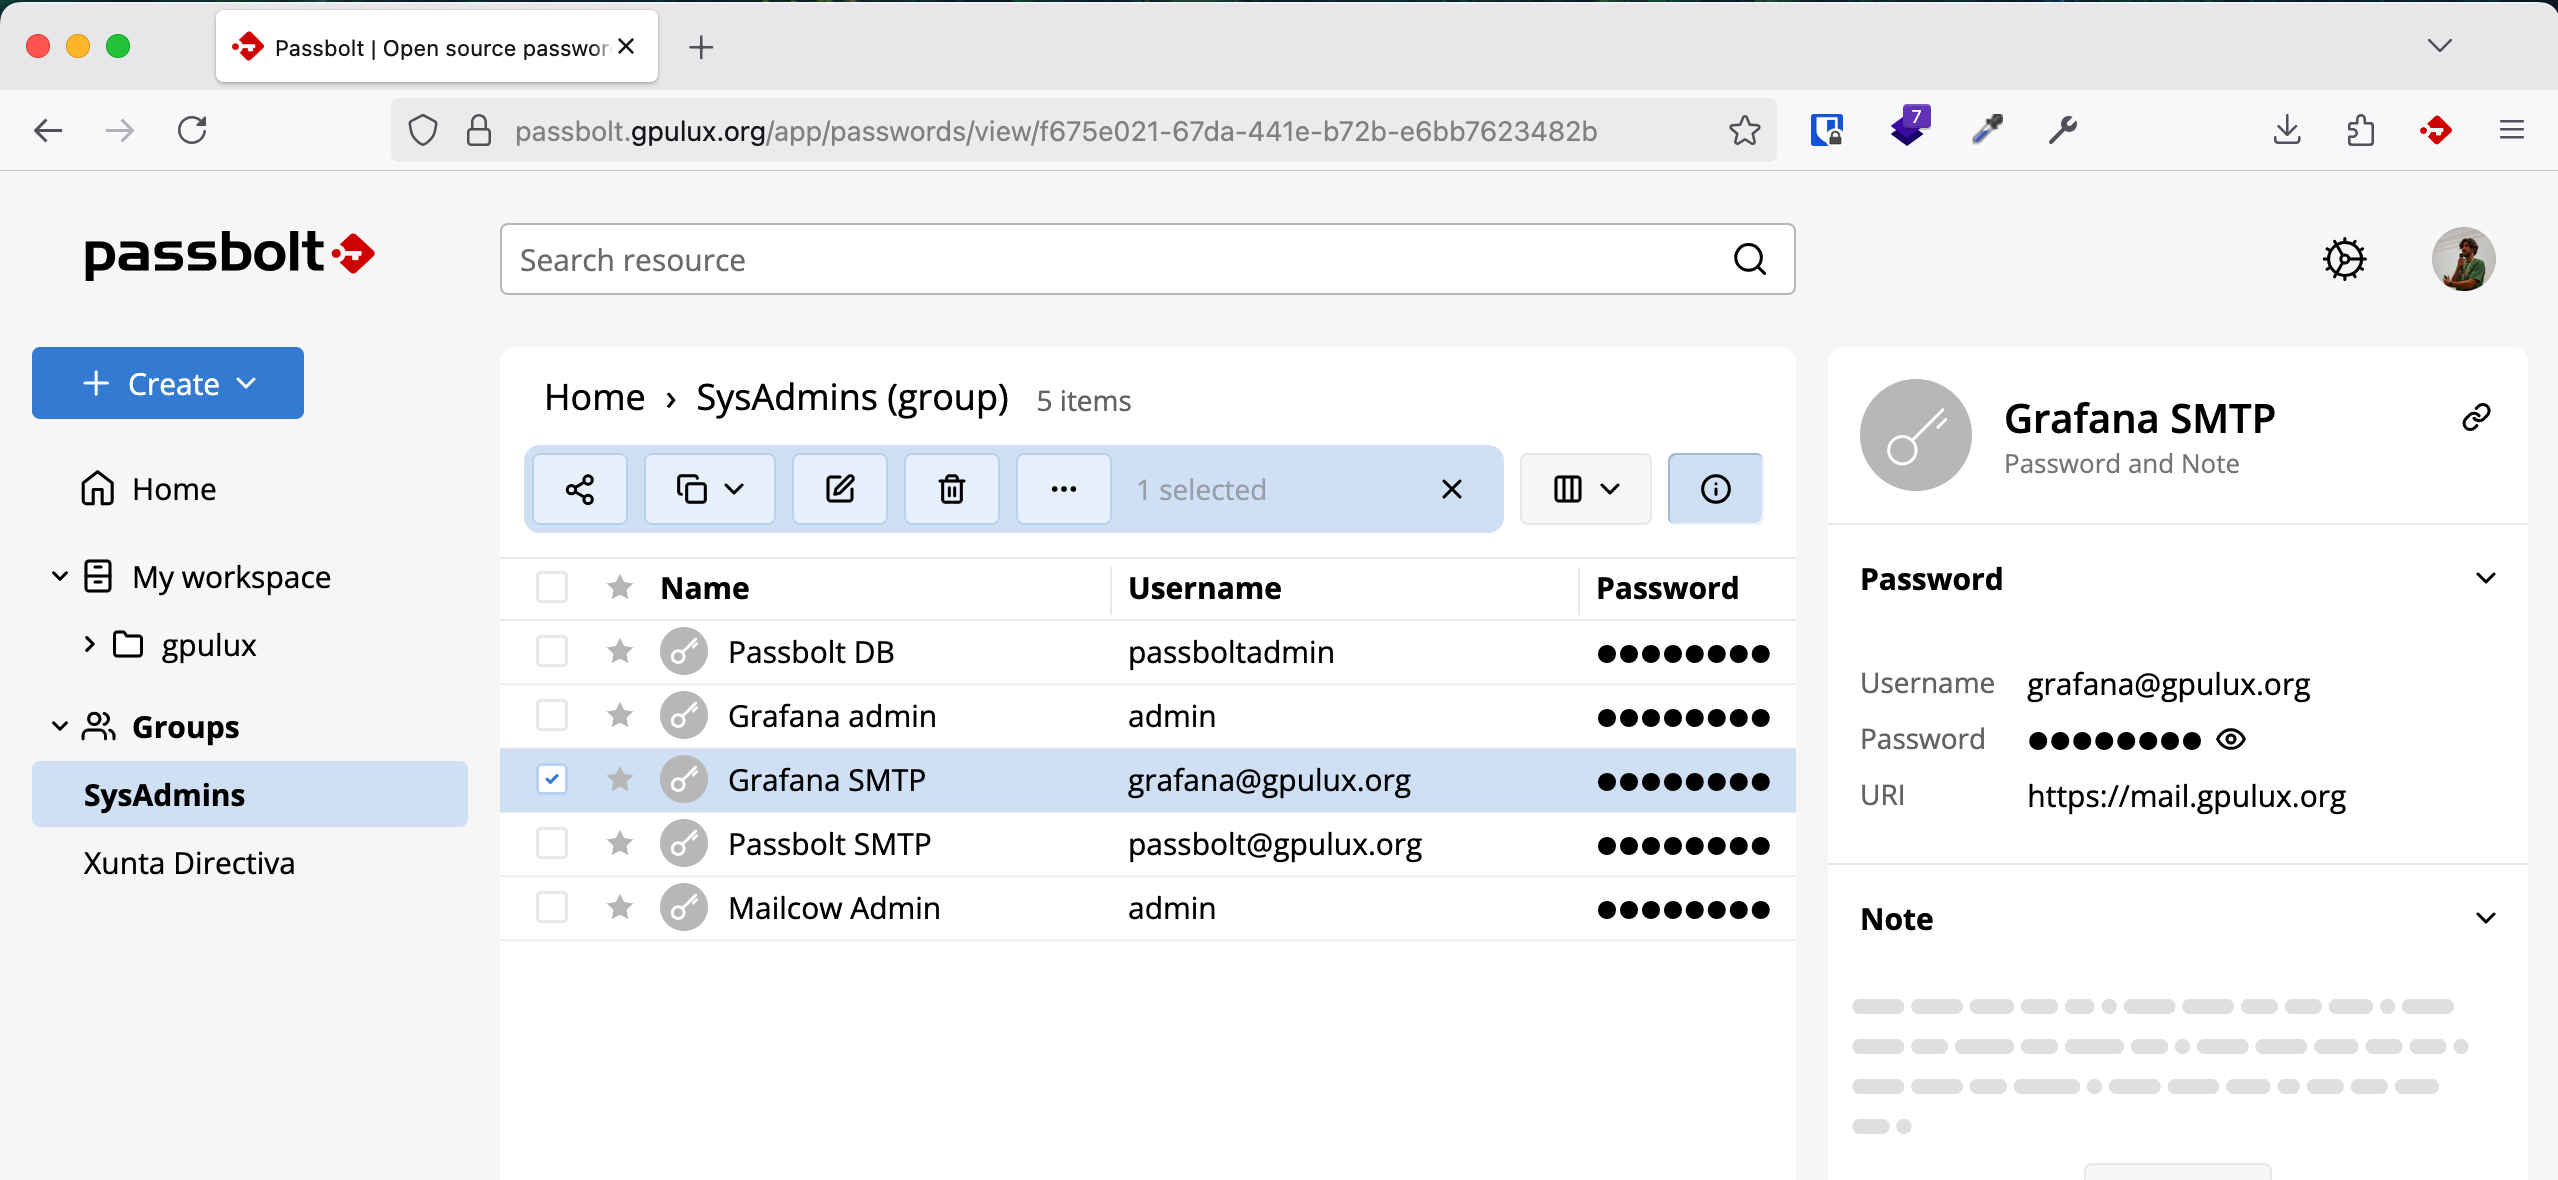
\includegraphics[width=\textwidth]{imaxes/passbolt-gpulux.png}
       \caption{Screenshot of the Passbolt web interface with stored credentials}
	\label{fig:passbolt-gpulux}
\end{figure}

\section{Mailing Lists with Mailman 3}

With the core services in place, the next step is to deploy the mailing list manager. Mailman 3 was chosen to replace the outdated Mailman 2.1 instance.

\subsection*{Mailman Container Setup}

A dedicated Incus container named \texttt{mailman} was created for this service using a Debian 12 image. The setup largely follows the official installation guides:
\begin{itemize}
    \item The official Debian installation guides for Mailman 3, downloaded with the official packages from the Debian repositories:
    \begin{itemize}
        \item \texttt{/usr/share/doc/mailman3/README.Debian}
        \item \texttt{/usr/share/doc/mailman3-web/README.Debian.gz}
        \item \texttt{/usr/share/doc/python3-mailman-hyperkitty/README.rst}
    \end{itemize}
    \item The online documentation for Mailman 3\cite{mailman3-docs}.
\end{itemize}

\begin{lstlisting}[language=bash,caption={Command to create the Mailman container}]
incus launch images:debian/12 mailman
\end{lstlisting}

Inside the container, the \texttt{mailman3-full} package was installed from the Debian repositories. This package bundles Mailman Core, the HyperKitty archiver, and Postorius for web-based list management. However, dependencies such as Postfix, Nginx, and Redis must be installed and configured separately to create a fully functional system.

\subsection*{Mailman Configuration}

The default configurations for Redis were sufficient for this deployment. For Nginx, the provided configuration file at \texttt{/etc/mailman3/nginx.conf} was linked at \texttt{/etc/nginx/ sites-enabled/}. The \texttt{server\_name} directive was set to \texttt{\_} to accept requests for any hostname, as Caddy handles the public-facing routing.

The most significant configuration was for Postfix. Since both Mailman and Mailcow operate under the same public IP address, they cannot simultaneously listen on the same standard email ports. To resolve this port conflict and to avoid duplicating email server setup (e.g., SPF, DKIM records), Mailman is configured to use Mailcow as a mail relay.

\begin{itemize}
    \item \textbf{Outgoing Mail:} All outgoing emails from Mailman are relayed through the Mailcow container. This is configured in Mailman's Postfix settings by setting \texttt{relayhost = [mailcow]:25}.
    \item \textbf{Incoming Mail:} Incoming mail for mailing lists (e.g., to \texttt{xunta@lists.gpulux.org}) is first received by Mailcow and then routed to Mailman's Postfix instance via LMTP. A transport map was added in Mailcow's UI to forward all mail for the \texttt{lists.gpulux.org} subdomain to the Mailman container's internal IP address. Mailcow's Postfix was also configured to trust relays from the local network.
\end{itemize}

This setup centralizes mail handling in Mailcow while allowing Mailman to manage the lists.

\subsection*{Data Migration}

The old mailing lists and their archives from the Mailman 2.1 instance were migrated following the official migration guide\cite{mailman3-migration}. The process involved exporting list configurations and archives from the old server and importing them into Mailman 3.

The following commands demonstrate the import process for a single list, \texttt{xunta@lists .gpulux.org}. The list configuration is imported first, followed by the message archive (\texttt{.mbox} file), and then the index is updated.

\begin{lstlisting}[language=bash,caption={Commands used to migrate a Mailman 2.1 list to Mailman 3}]
# Import list settings and subscribers
mailman --run-as-root import21 xunta@lists.gpulux.org /opt/mailman-data/config.pck

# Import message archive into HyperKitty
mailman-web hyperkitty_import -l xunta@lists.gpulux.org /opt/mailman-data/xunta.mbox

# Update the search index for the imported list
mailman-web update_index_one_list xunta@lists.gpulux.org
\end{lstlisting}

Figure~\ref{fig:mailman-ui} shows the HyperKitty web archiver after the migration, displaying the imported messages from an old mailing list.

\begin{figure}[h!]
	\centering
	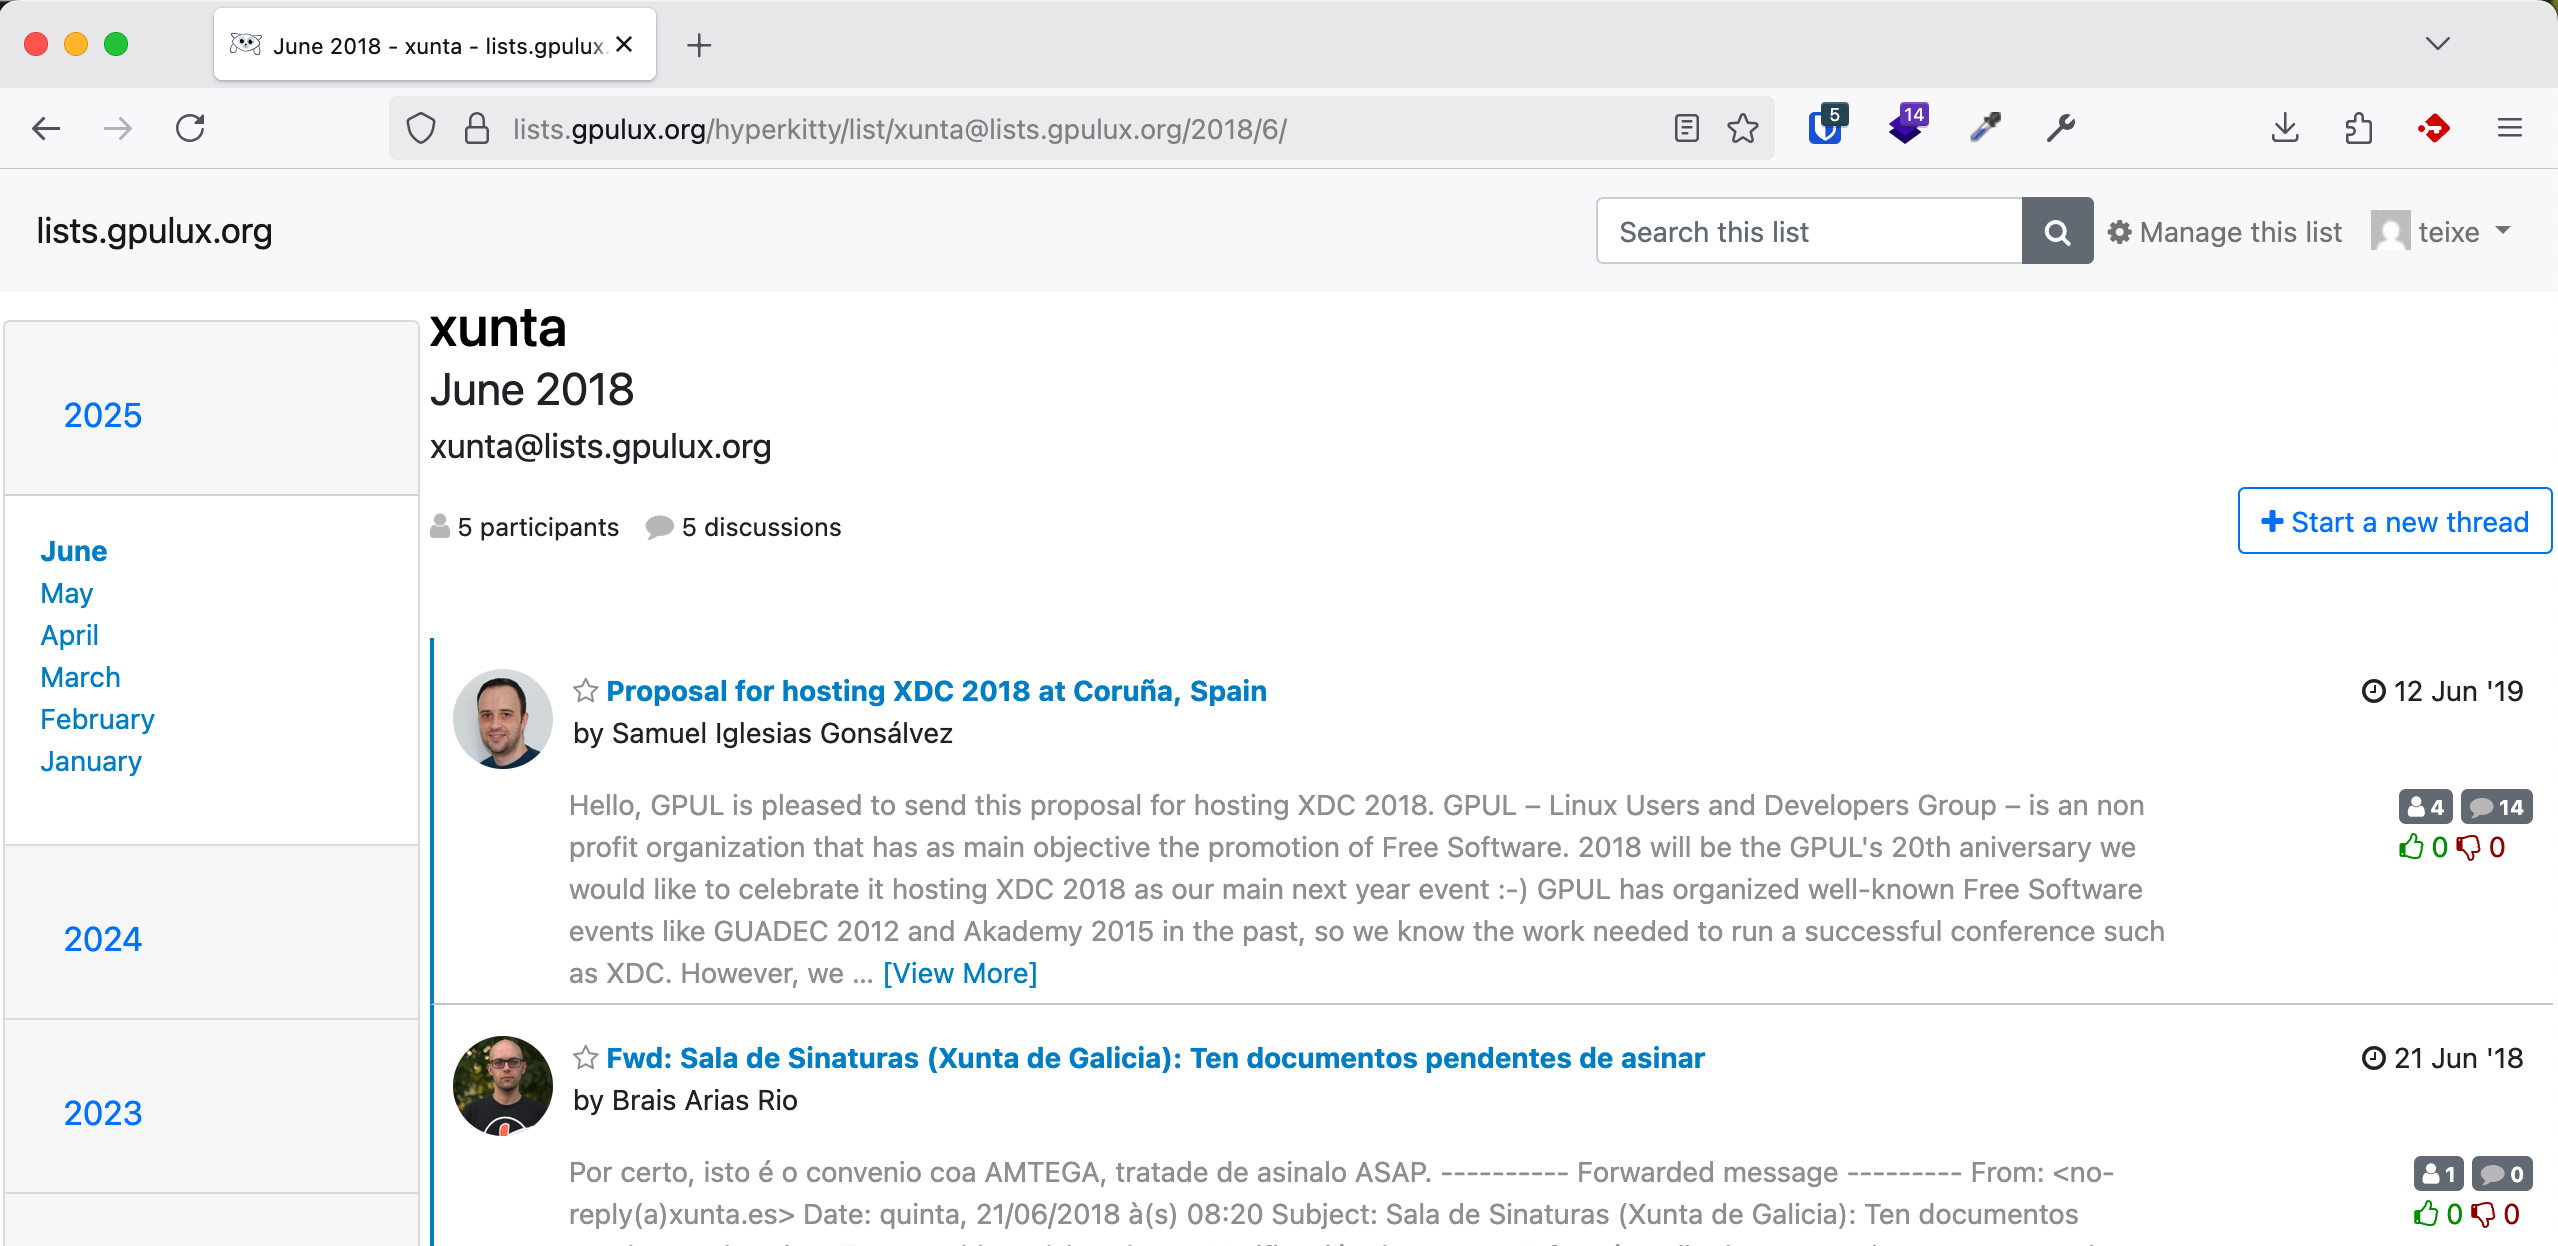
\includegraphics[width=\textwidth]{imaxes/hyperkitty-ui.png}
       \caption{Screenshot of HyperKitty displaying imported mailing list archives}
	\label{fig:mailman-ui}
\end{figure}

\subsection*{Log Management}

Since Mailman was installed from official Debian packages, log rotation is handled automatically. The packages provide configuration files at \texttt{/etc/logrotate.d/mailman3} and \texttt{/etc/logrotate.d/mailman3-web}, which ensure that log files are regularly rotated to prevent them from consuming excessive disk space.

These log files are forwarded to Loki by the Grafana Alloy agent, centralizing them with other system and application logs. The following configuration was added to scrape the Mailman log files:

\begin{lstlisting}[caption={Grafana Alloy configuration forwarding Mailman logs to Loki}]
loki.source.file "mailman" {
  targets    = [
    {__path__ = "/var/log/mailman3/mailman.log"},
    {__path__ = "/var/log/mailman3/web/mailman-web.log"},
  ]
  forward_to = [loki.write.local.receiver]
}
\end{lstlisting}

\subsection*{Reverse Proxy Configuration}

To expose Mailman's web interface (Postorius and HyperKitty), the Caddy reverse proxy is configured to forward requests for \texttt{lists.gpulux.org} to the Mailman container.

\begin{lstlisting}[caption={Caddyfile configuration used to expose Mailman 3 via the reverse proxy}]
lists.gpulux.org {
    reverse_proxy mailman:80
}
\end{lstlisting}

\section{Invoicing with FacturaScripts}

To handle the association's billing and financial records, FacturaScripts was chosen as the invoicing software. Its deployment provides a centralized platform for managing invoices, clients, and products, streamlining administrative workflows.

Following the established pattern, the service was deployed in a dedicated Incus container named \texttt{invoicing} using a Debian 12 image. The central Caddy reverse proxy was configured to expose the service at \texttt{facturas.gpulux.org}.

\subsection*{FacturaScripts Configuration}

The installation of FacturaScripts was performed following the official documentation\cite{facturascripts-install-linux}, which outlines the setup of a standard LAMP stack. MariaDB was used as the database server instead of MySQL.

To simplify the reverse proxy configuration, the application was installed directly in the web server's root directory (\texttt{/var/www/html}) instead of a subdirectory, avoiding the need for path rewrites. Apache's \texttt{remoteip} module was enabled to ensure that client IP addresses are correctly logged through the proxy.

Figure~\ref{fig:facturascripts-wizard} shows the FacturaScripts setup wizard after a successful installation.

\begin{figure}[H]
	\centering
	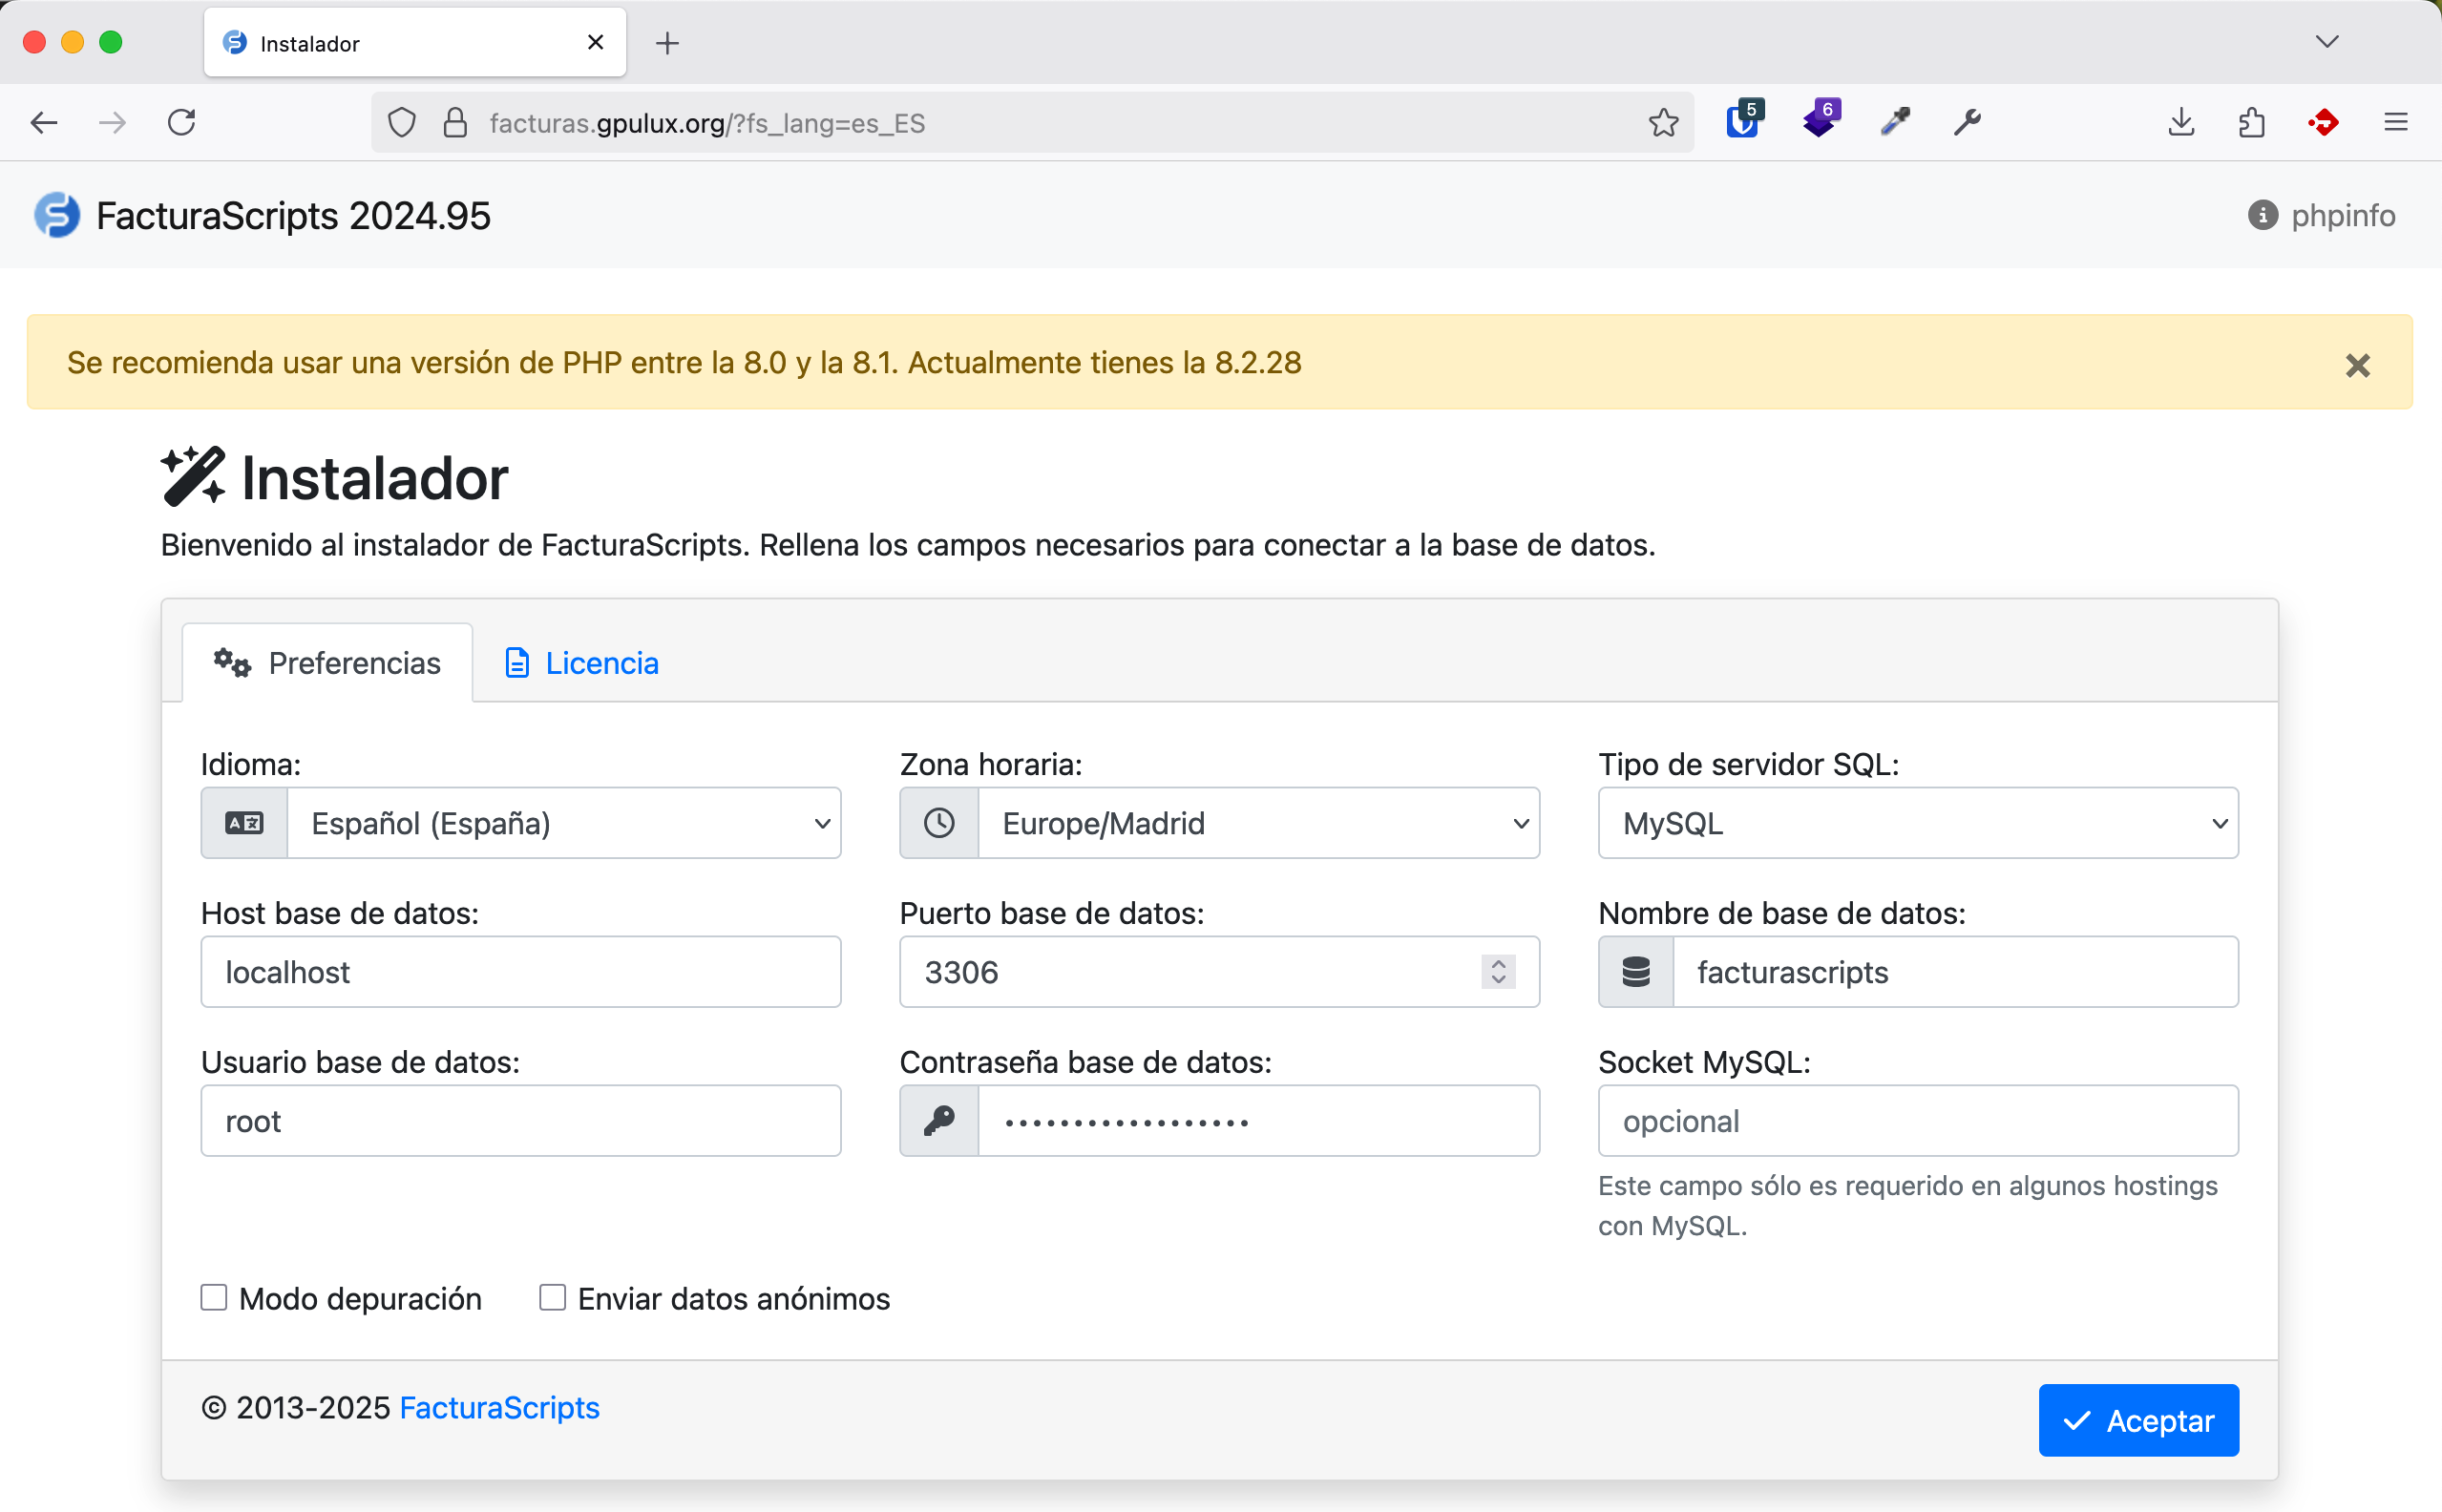
\includegraphics[width=\textwidth]{imaxes/facturascripts-wizard.png}
       \caption{Screenshot of the FacturaScripts setup wizard}
	\label{fig:facturascripts-wizard}
\end{figure}

\section{Event Management with Pretalx}

The next service to be deployed is Pretalx, the platform chosen for event management. In line with the infrastructure's design, the service was deployed in a dedicated Incus container named \texttt{pretalx} using a Debian 12 image. The installation was performed following the official documentation\cite{pretalx-install}, and the central Caddy reverse proxy was configured to expose the service at \texttt{pretalx.gpulux.org}.

\subsection*{Pretalx Configuration}

Inside the container, the only difference from the official documentation is that Nginx was configured to serve static files behind a reverse proxy for the main Pretalx application, which runs on a separate port. This setup is standard for web applications of this type.

\begin{lstlisting}[caption={Nginx configuration used by Pretalx to proxy the application and serve static files}]
server {
    listen 80 default_server;

    # Serve static files
    location /static/ {
        alias /var/pretalx/static/;
        expires 7d;
        access_log off;
    }

    # Serve uploaded media
    location /media/ {
        alias /var/pretalx/data/media/;
        expires 7d;
        add_header Content-Disposition 'attachment';
        access_log off;
    }

    # Proxy everything else
    location / {
        proxy_pass http://127.0.0.1:8345;
        proxy_set_header Host $http_host;
        proxy_set_header X-Real-IP $remote_addr;
        proxy_set_header X-Forwarded-For $proxy_add_x_forwarded_for;
        proxy_set_header X-Forwarded-Proto http;
    }
}
\end{lstlisting}

Figure~\ref{fig:pretalx-admin} shows the Pretalx administration dashboard, where organizers can manage event details, submissions, and schedules.

\begin{figure}[h!]
	\centering
	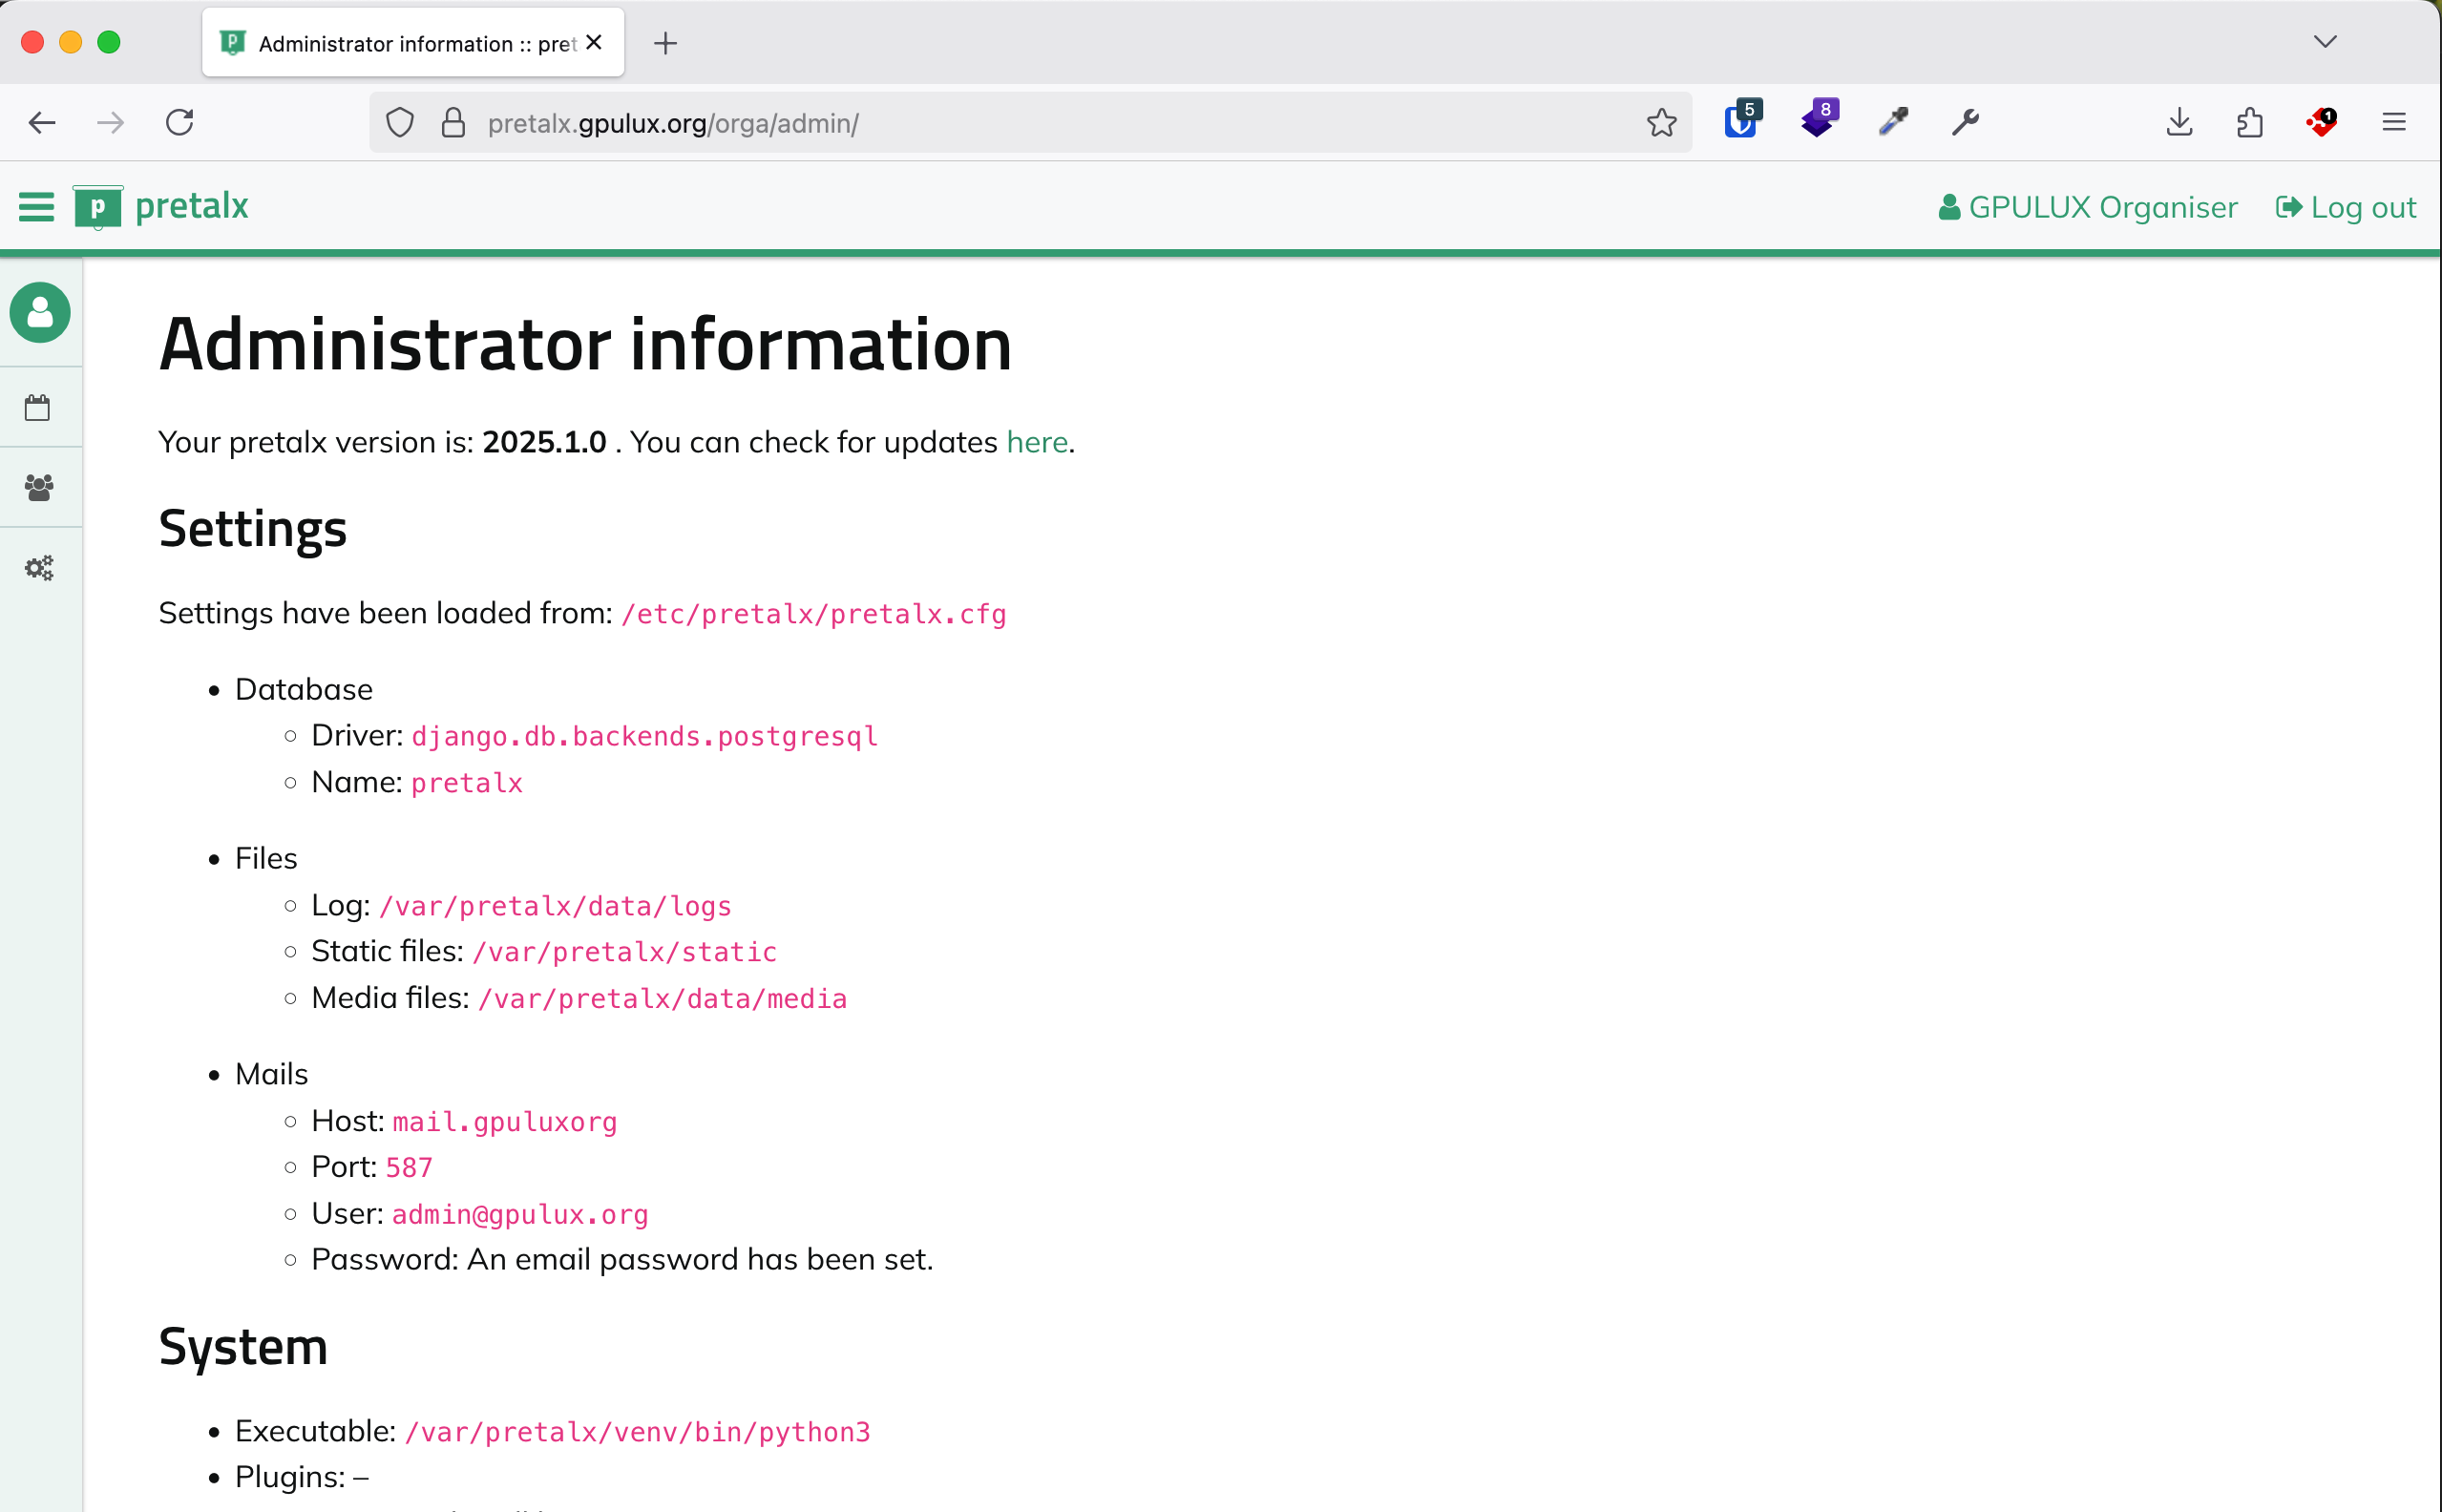
\includegraphics[width=\textwidth]{imaxes/pretalx-admin.png}
       \caption{Screenshot of the Pretalx administration dashboard}
	\label{fig:pretalx-admin}
\end{figure}

\section{Groupware with Nextcloud}

To provide file hosting, calendar, and contact management capabilities, Nextcloud was deployed as the primary groupware solution. The official Nextcloud All-in-One (AIO) Docker image\cite{nextcloud-aio} was used, which simplifies the installation and management of Nextcloud and its components, including Nextcloud Talk for video conferencing.

\subsection*{Nextcloud Container Setup}

Following the pattern of other Docker-based services, Nextcloud AIO runs within a dedicated Incus container with nesting enabled. A container named \texttt{nextcloud} was created from a Debian 12 image and configured to support Docker. The Caddy reverse proxy was configured to expose the Nextcloud instance at \texttt{cloud.gpulux.org}. The AIO stack runs the Apache web server in a container that listens on port 11000.

\begin{lstlisting}[language=bash,caption={Commands to create and configure the Nextcloud container}]
incus launch images:debian/12 nextcloud
incus config set nextcloud security.nesting=true
\end{lstlisting}

The installation is managed through a web interface provided by the AIO image. A temporary proxy device was created to expose the AIO interface during the initial setup, and was removed afterward.

\begin{lstlisting}[language=bash,caption={Commands to temporarily expose the Nextcloud AIO setup interface}]
incus config device add nextcloud nextcloud-aio proxy \
  listen=tcp:0.0.0.0:8080 connect=tcp:127.0.0.1:8080
\end{lstlisting}

\subsection*{Nextcloud Configuration}

The AIO web interface guides the administrator through the entire setup process, including domain configuration and the selection of optional components.

For Nextcloud Talk to function correctly, the TURN server requires port 3478 to be accessible over both TCP and UDP. Two proxy devices were added to the container to forward this traffic.

\begin{lstlisting}[language=bash,caption={Commands to forward the ports required for Nextcloud Talk}]
incus config device add nextcloud talk-stun-udp proxy \
  listen=udp:0.0.0.0:3478 connect=udp:127.0.0.1:3478

incus config device add nextcloud talk-stun-tcp proxy \
  listen=tcp:0.0.0.0:3478 connect=tcp:127.0.0.1:3478
\end{lstlisting}

\subsection*{Log Management}

As with other Dockerized services, logs from Nextcloud AIO are forwarded to Loki using the Docker logging driver. The Docker daemon inside the \texttt{nextcloud} container was configured with the same Loki driver settings used for Mailcow. This ensures that logs from all Nextcloud AIO containers are centralized in Grafana for monitoring and analysis.

\section{Real-Time Communication with Matrix}

For real-time communication, including instant messaging and voice/video calls, a Matrix homeserver was deployed. Synapse, the reference homeserver implementation from the Matrix Foundation, was chosen for this role. As with other services, Synapse was installed in a dedicated Incus container named \texttt{matrix} using a Debian 12 image. The Caddy reverse proxy was configured to expose the Matrix server following the official documentation\cite{matrix-caddy-reverse-proxy}.

\subsection*{Matrix Configuration}

The installation of Synapse was performed following its official documentation\cite{synapse-install-debian}. The \texttt{matrix-syn apse-py3} package was installed from the official Matrix repository. During the installation, PostgreSQL was configured as the database backend, as it is the recommended choice for production environments. The rest of the configuration was handled through the package installer configuration utility.

User registration is currently managed via a command-line script. While public registration is disabled for now, this can be changed in the future, and other methods like token-based registration can be implemented, among other options.

\begin{lstlisting}[language=bash,caption={Command used to register a new Matrix user}]
register_new_matrix_user -c /etc/matrix-synapse/homeserver.yaml http://localhost:8008
\end{lstlisting}

Figure~\ref{fig:element-example} shows the Element web client, a popular client for the Matrix protocol, being used for a conversation and a video call between two members of the association, demonstrating the successful deployment of the service.

\begin{figure}[H]
	\centering
	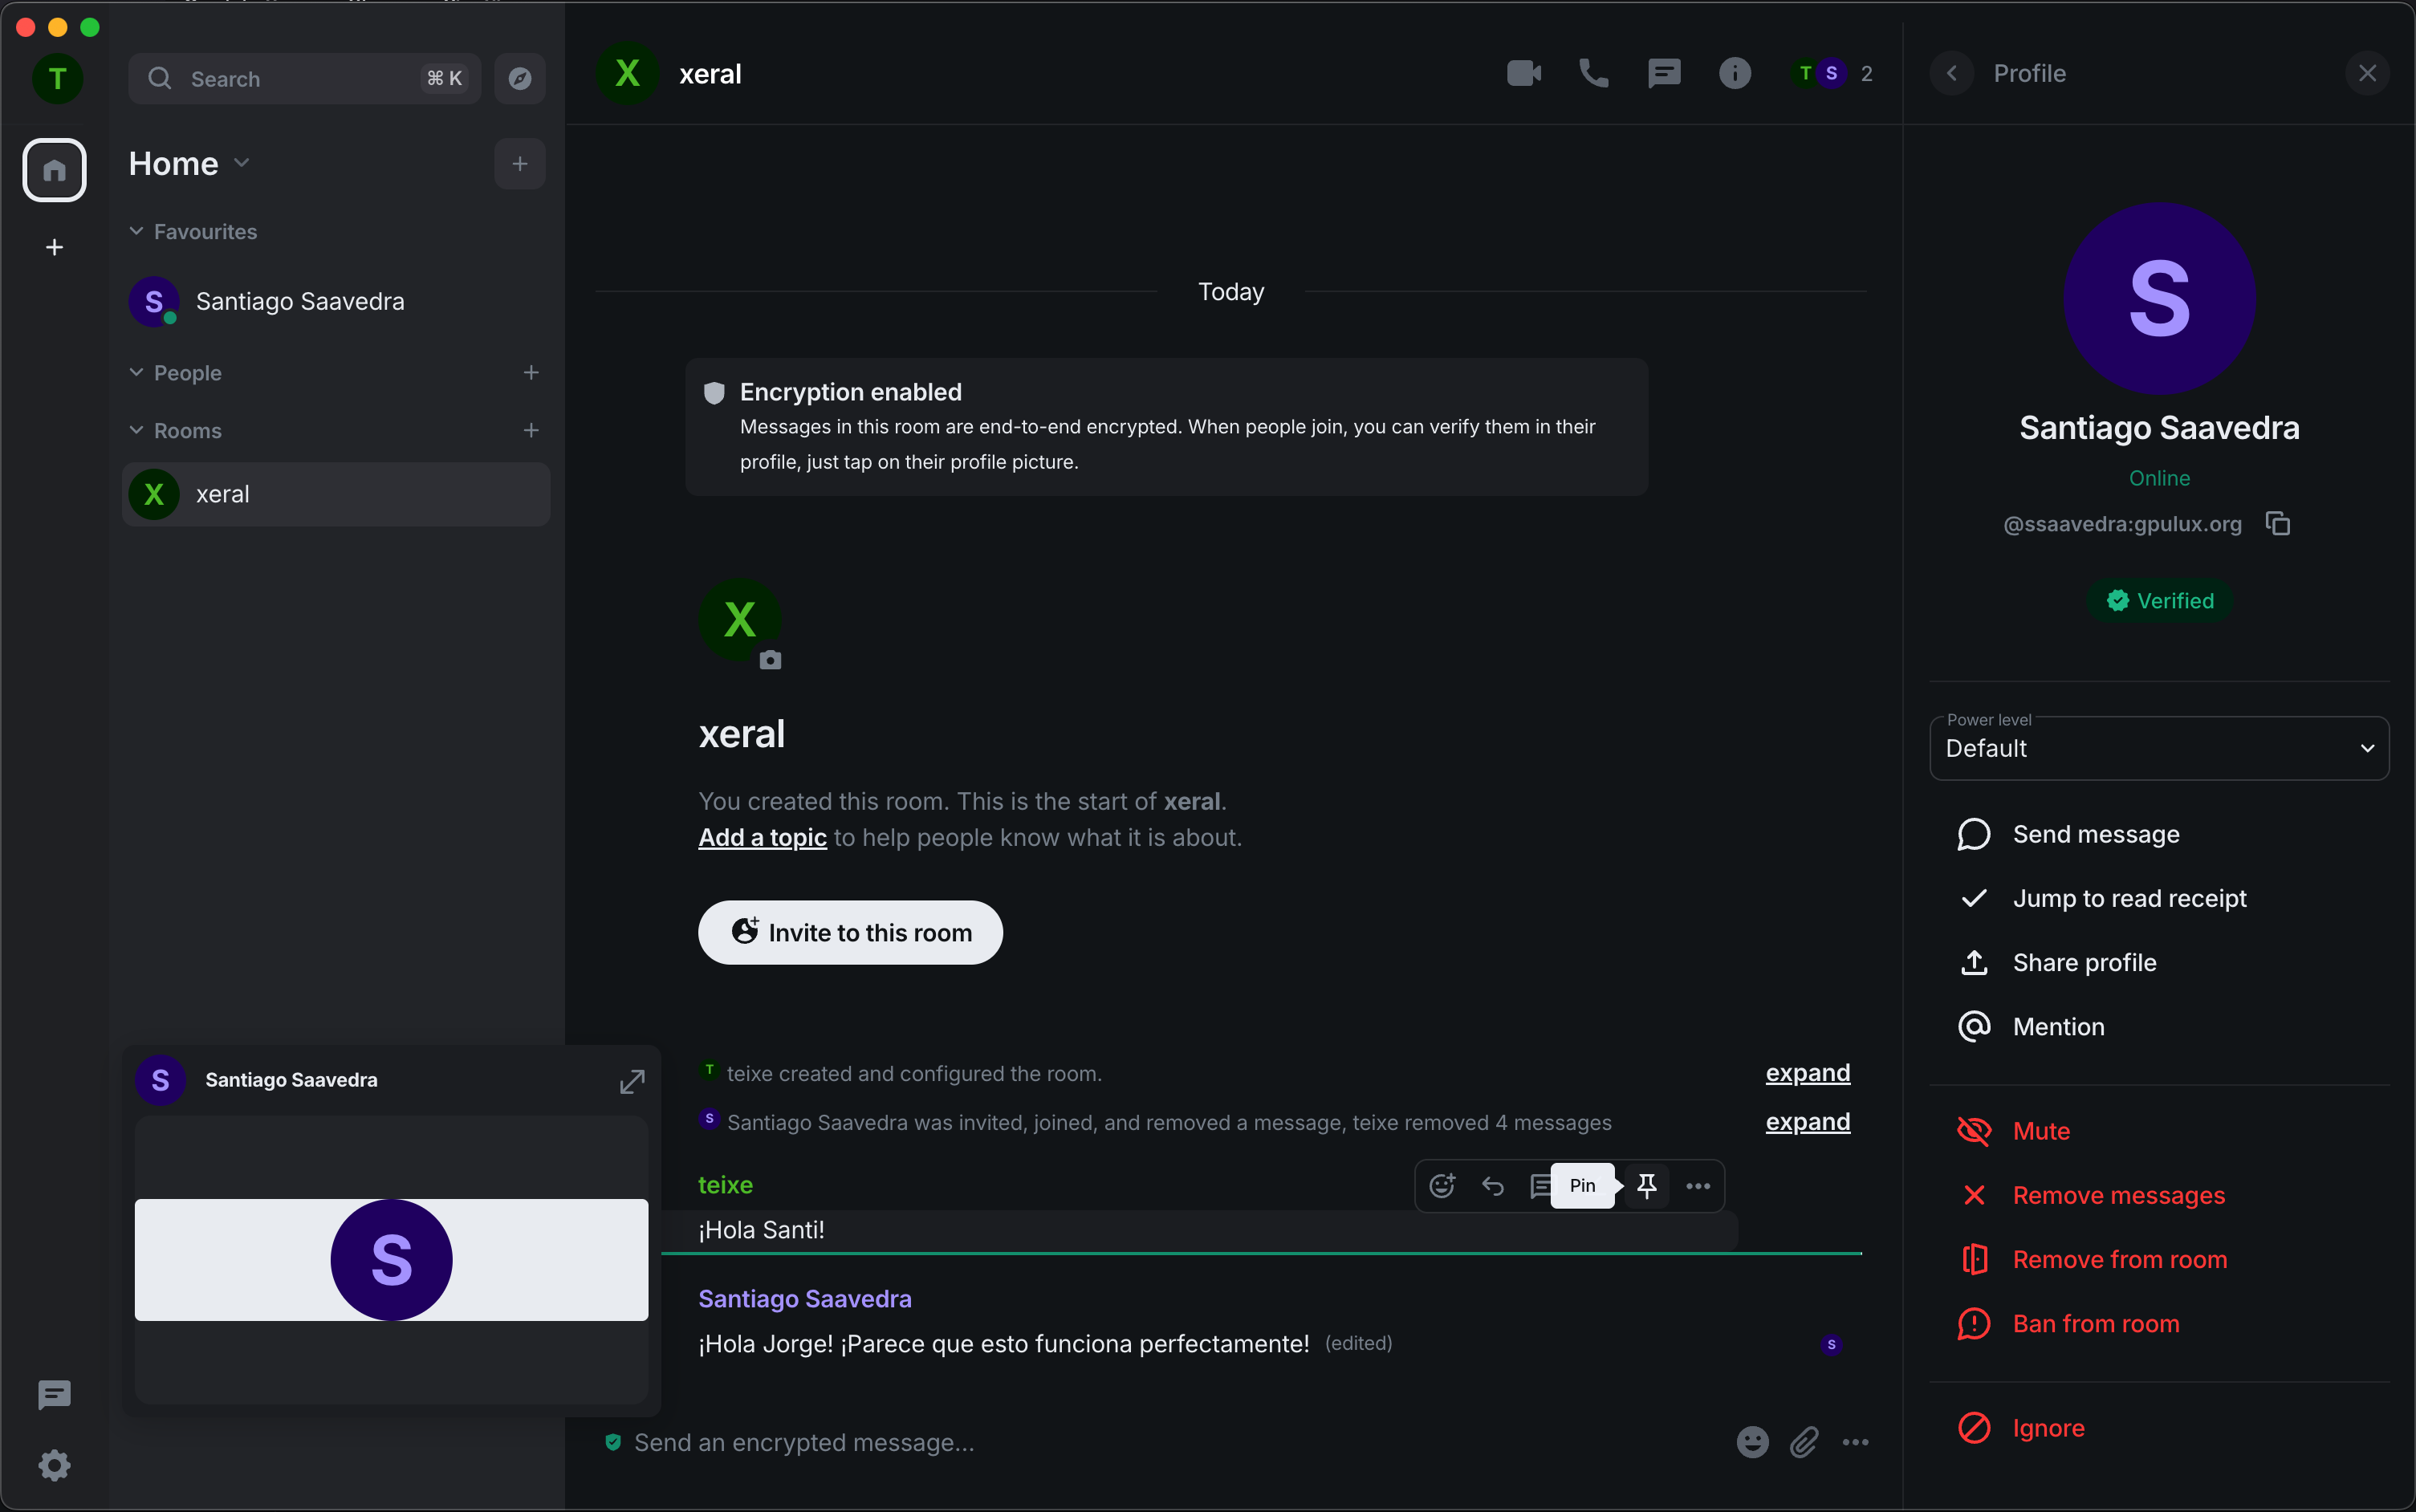
\includegraphics[width=\textwidth]{imaxes/element-example.png}
       \caption{Screenshot of the Element web client during a chat and video call}
	\label{fig:element-example}
\end{figure}

\section{Source Code Management with GitHub}

As established in the technology selection chapter, GitHub will continue to be used for the association's source code management. As a cloud-based service, this required no specific implementation on the new infrastructure.

\section{Backup Strategy}

Incus provides built-in utilities for creating and managing instance backups, primarily through snapshots\cite{incus-backup-docs}. These tools allow for point-in-time recovery and can be automated to run on a schedule. Key configuration options like \texttt{snapshots.schedule} and \texttt{snapshots.expiry} enable the creation of regular backups (e.g., daily or weekly) and define a retention policy to automatically delete old snapshots, preventing them from consuming excessive disk space.

However, a significant limitation of this approach is that snapshots are stored within the same Incus storage pool as the instances themselves. This means that a failure of the primary storage array would result in the loss of both the live data and its backups.

To address this and ensure backup reliability, a distributed storage strategy is employed. The instance snapshots are exported as compressed archives and distributed across a network of trusted, off-site locations. Several GPUL members have offered to collaborate by hosting these backups on their personal Network-Attached Storage (NAS) servers at home.

This distributed model provides a robust defense against data loss. In the future, this approach may be further enhanced by repurposing some of the old servers in the GPUL office to create a synchronized backup storage node, further centralizing and securing the backup process.
